%% =====================================================================
%% PoliTo DSML Lab — Credit-card default detection
%% IEEE conference template (IEEEtran V1.8b), UNMODIFIED.
%% Do NOT change the document class, fonts, or margins (exam rule: any
%% template modification => 0 points for the report). Max 4 pages excl.
%% references.
%%
%% Build: Overleaf (IEEEtran is built in) or any TeX Live with the
%% vendored IEEEtran.cls in this folder. Figures live in ./figures/.
%%
%% STATUS: Step-2 baseline draft. Sections marked "STEP 3" are stubs to be
%% completed with the rf_balanced + PAY-semantic feature-engineering story
%% (final LB 0.720/0.721). The baseline (HistGradientBoosting, LB 0.712) is
%% fully written and all its numbers are generated by
%%   python experiments/tune_baseline.py
%% =====================================================================
\documentclass[conference]{IEEEtran}

\usepackage{graphicx}
\usepackage{booktabs}
\usepackage{amsmath}
\usepackage{url}

\begin{document}

\title{Predicting Credit-Card Default under Class Imbalance:\\
A Threshold-Tuned Gradient-Boosting Approach}

% TODO(author): fill in name + student ID per the exam rules.
\author{\IEEEauthorblockN{Student Name}
\IEEEauthorblockA{Politecnico di Torino\\
Data Science and Machine Learning Laboratory\\
Email: student@studenti.polito.it}}

\maketitle

\begin{abstract}
We address the prediction of next-month credit-card default on the UCI
``default of credit card clients'' data, a binary classification task whose
strong class imbalance (about 22\% defaulters) makes raw accuracy misleading;
the task is therefore optimised for macro-F1. We build a leakage-free
scikit-learn pipeline that folds undocumented categorical codes, imputes and
encodes the features, and trains a histogram-based gradient-boosting classifier
whose decision threshold is tuned for macro-F1. This baseline reaches a
cross-validated macro-F1 of 0.708 and a public-leaderboard score of 0.712.
% TODO(Step 3): extend the abstract with the final model (balanced random
% forest + PAY-semantic feature engineering) and its 0.720/0.721 leaderboard
% result once those sections are written.
\end{abstract}

% =====================================================================
\section{Problem Overview}
% =====================================================================
The task is to predict whether a credit-card client will \emph{default} on
their next monthly payment, a binary classification problem
($0=\text{no default}$, $1=\text{default}$) on the UCI ``default of credit card
clients'' dataset~\cite{yeh2009, uci}. The full dataset describes 30{,}000
clients in Taiwan. For this project it is split into a labelled
\emph{development} set of 24{,}000 clients, used for all training and
cross-validation, and an unlabelled \emph{evaluation} set of 6{,}000 clients
whose predictions are scored on the course leaderboard.

Each client is described by 23 features: the credit limit (\texttt{LIMIT\_BAL}),
demographics (\texttt{SEX}, \texttt{EDUCATION}, \texttt{MARRIAGE}, \texttt{AGE}),
six months of repayment status (\texttt{PAY\_0}, \texttt{PAY\_2}--\texttt{PAY\_6}),
six monthly bill statements (\texttt{BILL\_AMT1}--\texttt{6}) and six monthly
payment amounts (\texttt{PAY\_AMT1}--\texttt{6}). \texttt{SEX},
\texttt{EDUCATION} and \texttt{MARRIAGE} are nominal; the remaining features,
including the repayment-status codes, are numeric/ordinal.

The data contains documented and undocumented quirks that the preprocessing must
handle. \texttt{EDUCATION} contains the undocumented codes $\{0,5,6\}$ (the
specification documents only $1$--$4$) and \texttt{MARRIAGE} contains the
undocumented code $\{0\}$ (documented $1$--$3$); both are folded into the
existing ``other'' category. The repayment-status columns take values in
$\{-2,-1,0,1,\dots,9\}$, where the specification only documents $-1$ (paid duly)
and $1$--$9$ (months of delay): in practice $-2$ (no consumption) and $0$
(revolving credit) also occur and carry distinct meaning, a point we exploit
later.

\textbf{Class imbalance and metric.} The development set is imbalanced: about
77.9\% of clients do not default and only 22.1\% do. Under this skew, a trivial
classifier that always predicts ``no default'' would already score about 78\%
accuracy while being useless for the minority class that matters. We therefore
optimise \textbf{macro-F1}~\cite{hegarcia2009}, the unweighted mean of the
per-class F1 scores, which
weights the default and non-default classes equally and rewards correctly
recovering the minority (default) class.

% =====================================================================
\section{Proposed Approach}
% =====================================================================
The model is a single scikit-learn~\cite{sklearn} \texttt{Pipeline} so that every fitted
transform sees only the training folds during cross-validation, guaranteeing no
information leaks from validation or evaluation data. The pipeline chains
code-folding, optional feature engineering and encoding, a column-wise
preprocessor, the estimator, and a final macro-F1 threshold tuner.

\subsection{Preprocessing}
\label{sec:preprocessing}
Cleaning is a \emph{stateless, deterministic} mapping (it fits nothing), so it is
inherently leakage-free: the undocumented \texttt{EDUCATION} codes $\{0,5,6\}$
are folded to $4$ and the undocumented \texttt{MARRIAGE} code $\{0\}$ to $3$,
collapsing them into the documented ``other'' buckets.

The remaining preprocessing is a \texttt{ColumnTransformer} with two branches.
Numeric features are median-imputed (a guard against unexpected missing values,
including any produced by guarded division in engineered features) and optionally
standardised. The three nominal features (\texttt{SEX}, \texttt{EDUCATION},
\texttt{MARRIAGE}) are most-frequent-imputed and one-hot encoded, with unknown
categories ignored at transform time so the evaluation set never breaks the
encoder. The repayment-status columns are kept as ordinal numeric inputs rather
than one-hot encoded, since their ordering carries the delinquency signal.

Standardisation is treated as a \emph{per-estimator} switch. A monotone
per-feature rescaling such as \texttt{StandardScaler} leaves a tree-based model
unchanged, because a tree only depends on the order of split points; we verified
this is bit-identical for the gradient-boosting model. The scaler is therefore
dropped on the tree path as a cost-free simplification and retained only when a
linear model needs it.

\subsection{Model Selection}
\label{sec:model-selection}
As a first strong baseline we compare three estimators of increasing capacity
under identical preprocessing and cross-validation: a stratified random
classifier (a floor), a class-balanced logistic regression (an interpretable
linear baseline), and a histogram-based gradient-boosting classifier (HGB). A
gradient-boosted decision tree is a natural first choice for this problem: it is
a strong off-the-shelf learner for heterogeneous tabular data, captures
non-linear interactions among the repayment, bill and payment histories without
manual feature crossing, is insensitive to feature scaling and monotone
transforms, and handles the mixed numeric/categorical inputs robustly. As shown
in Section~\ref{sec:results}, HGB is the best of the three baselines, so it
anchors the rest of the study.

% ---------------------------------------------------------------------
% STEP 3: extend Model Selection with the full bake-off and the chosen model.
%  - Bake-off HGB vs RandomForest vs LogisticRegression (diversity / decorrelation).
%  - Imbalance handling: class_weight="balanced" RandomForest (rf_balanced), LB 0.713.
%  - PAY-semantic feature engineering on RF (paysem/util/payratio, stress) -> LB 0.720/0.721.
%  - State the deployed model = config.yaml `chosen` = what main.py writes (gold rule).
% ---------------------------------------------------------------------

\subsection{Hyperparameter Tuning}
\label{sec:tuning}
All model selection and tuning is performed with stratified 5-fold
cross-validation (\texttt{StratifiedKFold}, shuffled, fixed seed) on the
development set, and is kept out of the submission entry point: \texttt{main.py}
only trains the single chosen configuration.

\textbf{Deployed objective.} Because the final classifier submits behind a tuned
decision threshold, we do not score candidates at the default $0.5$ cut. Instead,
for each fold we obtain out-of-fold class probabilities and select the threshold
that maximises macro-F1 over a grid of 181 values spanning $0.05$ to $0.95$. This
\emph{threshold-at-best-macro-F1} on out-of-fold probabilities is the objective
every experiment reports, matching what the deployed model does. In production the
threshold is set by \texttt{TunedThresholdClassifierCV}, which chooses it on inner
cross-validation folds only, so the operating point is selected without leakage.

Threshold tuning is itself a sizeable, free gain: it lifts the baseline HGB
macro-F1 from $0.687$ at the $0.5$ cut to $0.708$ at the tuned threshold
($\approx 0.31$), an improvement of about $+0.021$ obtained without changing the
model. A randomised search over the HGB hyperparameters (learning rate, number of
iterations, tree size, regularisation) yielded only a marginal cross-validated
gain ($\le +0.003$ macro-F1) that did not justify departing from the library
defaults for the baseline; the substantial improvements came instead from the
model family and feature engineering developed in Section~\ref{sec:model-selection}.

% =====================================================================
\section{Results}
\label{sec:results}
% =====================================================================
Table~\ref{tab:baseline} reports the three baselines under the deployed objective:
5-fold cross-validated macro-F1 at each model's own tuned threshold, plus
ROC-AUC. The gradient-boosting model is clearly the strongest baseline, and its
cross-validated macro-F1 of $0.708$ corresponds to a public-leaderboard score of
\textbf{0.712}.

\begin{table}[t]
\caption{Baseline comparison (5-fold CV, macro-F1 at each model's tuned
threshold). HGB is the deployed baseline; its public leaderboard score is 0.712.}
\label{tab:baseline}
\centering
\begin{tabular}{lcc}
\toprule
Model & CV macro-F1 & ROC-AUC \\
\midrule
Stratified dummy            & 0.506 & 0.506 \\
Logistic regression (balanced) & 0.695 & 0.728 \\
\textbf{HistGradientBoosting} & \textbf{0.708} & \textbf{0.783} \\
\bottomrule
\end{tabular}
\end{table}

The baseline confusion matrix at the tuned threshold (Fig.~\ref{fig:cm-baseline})
makes the imbalance trade-off concrete. Per-class metrics at this operating point
are: non-default precision/recall/F1 $=0.869/0.878/0.873$ and default
precision/recall/F1 $=0.553/0.532/0.543$. The tuned threshold deliberately trades
some non-default accuracy to recover roughly half of the true defaulters, which is
what macro-F1 rewards.

\begin{figure}[t]
\centering
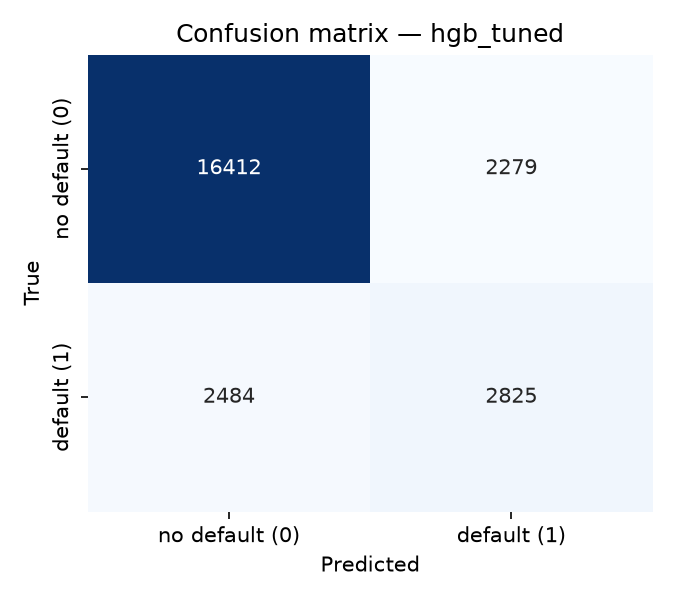
\includegraphics[width=0.86\columnwidth]{figures/cm_baseline.png}
\caption{Baseline HistGradientBoosting confusion matrix (out-of-fold, tuned
threshold $\approx 0.31$) on the 24{,}000-client development set.}
\label{fig:cm-baseline}
\end{figure}

% ---------------------------------------------------------------------
% STEP 3: extend Results with the milestone table and final confusion matrix.
%  - CV macro-F1 + public-LB milestone table: HGB 0.712 -> rf_balanced 0.713
%    -> +payratio 0.716 -> paysem combos 0.719/0.720 -> 0.721.
%  - Final-model confusion matrix + per-class metrics.
%  - The two final picks (A 0.720, B 0.721) and that only the private LB counts.
% ---------------------------------------------------------------------

% =====================================================================
\section{Discussion}
% =====================================================================
% STEP 3 stub. To be written:
%  - Error analysis: where the model still confuses default vs non-default.
%  - CV<->LB decoupling on this dataset and how candidates were ranked by the LB.
%  - RF-vs-HGB behaviour on engineered features (why FE helped RF, not HGB).
%  - Limitations; one-line out-of-syllabus motivation if any method is off-syllabus.
A detailed error analysis and discussion of the cross-validation--leaderboard
relationship are developed alongside the final model.

% =====================================================================
\begin{thebibliography}{9}
% =====================================================================
\bibitem{yeh2009}
I.-C. Yeh and C.-H. Lien, ``The comparisons of data mining techniques for the
predictive accuracy of probability of default of credit card clients,''
\emph{Expert Systems with Applications}, vol.~36, no.~2, pp.~2473--2480, 2009.

\bibitem{uci}
UCI Machine Learning Repository, ``Default of credit card clients data set,''
\url{https://archive.ics.uci.edu/dataset/350/default+of+credit+card+clients}.

\bibitem{sklearn}
F. Pedregosa \emph{et al.}, ``Scikit-learn: Machine learning in Python,''
\emph{Journal of Machine Learning Research}, vol.~12, pp.~2825--2830, 2011.

\bibitem{hegarcia2009}
H. He and E. A. Garcia, ``Learning from imbalanced data,'' \emph{IEEE
Transactions on Knowledge and Data Engineering}, vol.~21, no.~9,
pp.~1263--1284, 2009.
\end{thebibliography}

\end{document}
